\documentclass[11pt,a4paper]{article}

\usepackage[margin=2.4cm]{geometry}
\usepackage{amsmath}
\usepackage{amssymb}
\usepackage{graphicx}
\usepackage{booktabs}
\usepackage{longtable}
\usepackage{array}
\usepackage{float}
\usepackage{caption}
\usepackage[table]{xcolor}
\usepackage{hyperref}
\hypersetup{colorlinks=true,linkcolor=black,citecolor=black,urlcolor=blue}

\newcommand{\degC}{\,^{\circ}\mathrm{C}}
\newcommand{\unit}[1]{\,\mathrm{#1}}

\title{\textbf{Flight Readiness Review --- Payload Thermal Analysis (v2)}\\[2mm]
\large High-Altitude Balloon Event-Camera Payload\\[1mm]
\normalsize Operating concept: on-board computer powered at 16 km}
\author{Thermal Analysis --- Systems Engineering}
\date{\today}

\begin{document}
\maketitle

\begin{abstract}
\noindent This report documents the thermal model and flight-readiness assessment of
the high-altitude balloon (HAB) event-camera payload for the operating concept in which
the on-board computer (OBC) is powered only on reaching the imaging altitude of
$16\unit{km}$. A coupled three-block model (external environment, enclosure-wall
conduction, and a two-dimensional planar internal field) is solved over the
ascent-to-apogee mission window from a cold-night initial temperature of $+5\degC$.
The internal cavity is modelled as a planar $(x,z)$ cross-section of the full
$170\unit{mm}$ interior width, capturing the left-right asymmetric component layout
without invoking axial symmetry. The component set reflects the mechanical CAD bill
of materials; storage peripherals (SSD, USB stick, SD card reader) absent from the
CAD are excluded. All ten payload components remain within their operating temperature
limits throughout the analysed window. The minimum cold-side margin is $+15.0\degC$
and the tightest hot-side margin is $+8.7\degC$ (Wolfgang GA100). The thermal design
is assessed \textbf{GO} for flight.
\end{abstract}

\tableofcontents
\bigskip

% ============================================================
\section{System Description and Geometry}
% ============================================================
The payload is housed in a cylindrical expanded-polypropylene (EPP) Thermobox enclosure.
The internal cavity is modelled as a two-dimensional planar $(x,z)$ section of full
width $W_{int}$ and height $H_{int}$, extruded to an out-of-plane slab depth $D_{int}$
for the volumetric energy balance. The outer enclosure shell is physically cylindrical,
and the outer geometry ($R_{box}$, $D_{box}$, $L_{box}$) is retained for the external
convection calculation in Block~A. The internal field is solved on a Cartesian
$(x,z)$ mesh covering the full cavity width from left wall to right wall; no
axial-symmetry assumption is applied, and both lateral walls appear as independent
Dirichlet boundaries. The geometry is summarised in Table~\ref{tab:geom}.

\begin{table}[H]
\centering
\caption{Enclosure geometry. Internal dimensions describe the planar meshed domain;
external dimensions are used for the Block~A convection calculation only.}
\label{tab:geom}
\begin{tabular}{llr}
\toprule
Symbol & Quantity & Value \\
\midrule
$W_{int}$ & Internal cavity width (planar $x$-extent)   & $0.170\unit{m}$ \\
$H_{int}$ & Internal cavity height                       & $0.250\unit{m}$ \\
$D_{int}$ & Out-of-plane slab depth                      & $0.170\unit{m}$ \\
$L_{wall}$& Side-wall thickness (EPP)                    & $0.030\unit{m}$ \\
$L_{cap}$ & End-cap thickness (EPP)                      & $0.030\unit{m}$ \\
$R_{box}$ & Outer radius (convection reference)          & $0.115\unit{m}$ \\
$L_{box}$ & Outer height                                 & $0.310\unit{m}$ \\
$D_{box}$ & Outer diameter (convection)                  & $0.230\unit{m}$ \\
\bottomrule
\end{tabular}
\end{table}

\begin{figure}[H]
\centering
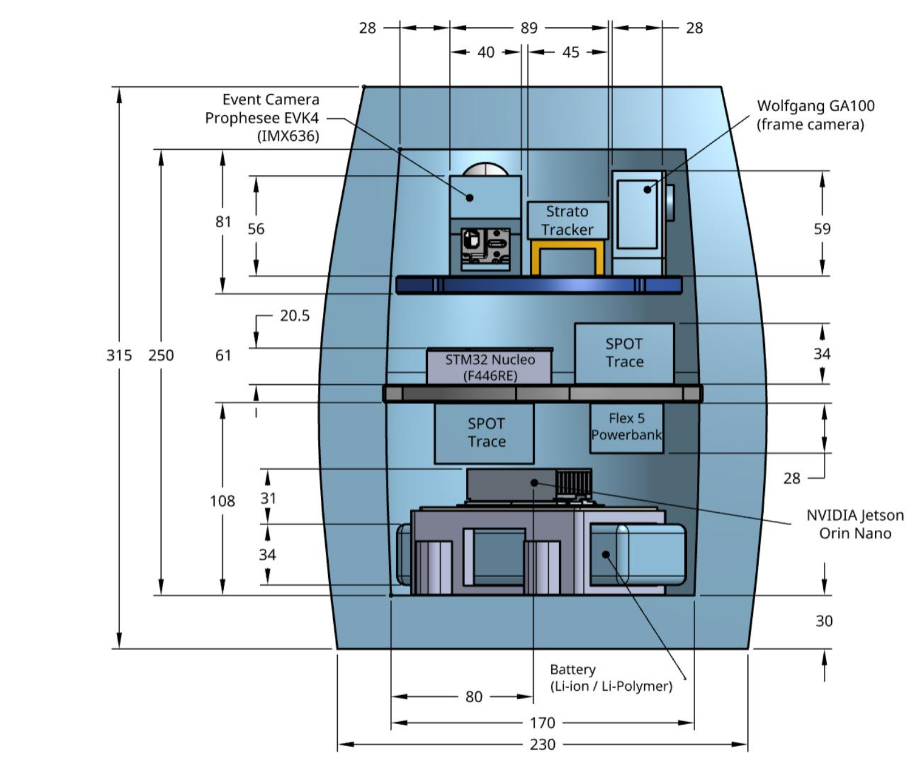
\includegraphics[width=0.62\textwidth]{cad_section.png}
\caption{Mechanical CAD section used as the reference layout for the meshed model.
The interior resolves four stacked bays: the camera bay on top (EVK4 left, Strato
Tracker centre, GA100 right), two mid-deck rows (STM32 upper-left with SPOT Trace,
Flex~5 powerbank lower-right with SPOT Trace), and the bottom bay (battery below in
a PETG cage, Jetson carrier board and SoC above in a stacked topology).
Components are mounted with clearance to the side walls.}
\label{fig:cad}
\end{figure}

% ============================================================
\section{Modelling Methodology}
% ============================================================
The model is decomposed into three coupled blocks. Block~A provides the external
free-stream temperature and convective coefficient as a function of altitude and
ascent velocity. Block~B solves transient conduction through the enclosure wall and
end caps. Block~C solves the two-dimensional planar temperature field of the internal
cavity, driven by the component heat loads and bounded by the Block~B wall temperatures.
The blocks are advanced with a lagged coupling each timestep.

% ------------------------------------------------------------
\subsection{Block A --- External Environment and Forced Convection}
% ------------------------------------------------------------
The ambient state is evaluated with the US Standard Atmosphere 1976, piecewise by
layer. Within a layer of base altitude $h_b$, base temperature $T_b$, base pressure
$P_b$ and lapse rate $L_b$,
\begin{equation}
T(h) = T_b + L_b\,(h-h_b),
\end{equation}
\begin{equation}
P(h) =
\begin{cases}
P_b\left(\dfrac{T}{T_b}\right)^{-g/(L_b R)}, & L_b \neq 0,\\[3mm]
P_b\,\exp\!\left(-\dfrac{g\,(h-h_b)}{R\,T_b}\right), & L_b = 0,
\end{cases}
\qquad
\rho = \frac{P}{R\,T},
\end{equation}
with $g=9.80665\unit{m/s^2}$ and $R=287.058\unit{J/(kg\,K)}$. Transport properties use
Sutherland-type fits,
\begin{equation}
\mu(T) = \frac{1.458\times10^{-6}\,T^{3/2}}{T+110.4},
\qquad
k_{air}(T) = \frac{2.495\times10^{-3}\,T^{0.8646}}{1 + 245.4\cdot 10^{-12/T}/T},
\qquad
\mathrm{Pr} = \frac{\mu\,c_p}{k_{air}}.
\end{equation}

The enclosure is treated as a cylinder in cross-flow at the ascent velocity $V$. The
Reynolds number and the Churchill--Bernstein Nusselt-number correlation give the
external convective coefficient:
\begin{equation}
\mathrm{Re} = \frac{\rho\,V\,D_{box}}{\mu},
\end{equation}
\begin{equation}
\mathrm{Nu} = 0.3 +
\frac{0.62\,\mathrm{Re}^{1/2}\,\mathrm{Pr}^{1/3}}
{\left[\,1+(0.4/\mathrm{Pr})^{2/3}\,\right]^{1/4}}
\left[\,1+\left(\frac{\mathrm{Re}}{282\,000}\right)^{5/8}\,\right]^{4/5},
\qquad
h_{ext} = \frac{\mathrm{Nu}\,k_{air}}{D_{box}}.
\end{equation}

% ------------------------------------------------------------
\subsection{Block B --- One-Dimensional Wall Conduction}
% ------------------------------------------------------------
Each wall segment (side, top cap, bottom cap) is discretised into $N$ nodes across the
thickness, with spacing $\Delta x = L_{wall}/(N-1)$. Transient conduction is advanced
with implicit Euler in a finite-volume form. Boundary nodes carry half control volumes;
interior nodes carry full control volumes. The outer surface (node $0$) exchanges with
the atmosphere through $h_{ext}$ and the inner surface (node $N-1$) with the cavity air
through the internal coefficient $h_{int}$:
\begin{align}
\text{Outer:}\quad &
\frac{\rho c_p \tfrac{\Delta x}{2}}{\Delta t}\left(T_0^{n+1}-T_0^{n}\right)
= h_{ext}\left(T_\infty - T_0^{n+1}\right)
  + \varepsilon\sigma\!\left(T_{sink}^{4}-\left(T_0^{n+1}\right)^{4}\right)
  + \frac{k}{\Delta x}\left(T_1^{n+1}-T_0^{n+1}\right),\\[1mm]
\text{Interior:}\quad &
\frac{\rho c_p \Delta x}{\Delta t}\left(T_i^{n+1}-T_i^{n}\right)
= \frac{k}{\Delta x}\left(T_{i-1}^{n+1}-2T_i^{n+1}+T_{i+1}^{n+1}\right),\\[1mm]
\text{Inner:}\quad &
\frac{\rho c_p \tfrac{\Delta x}{2}}{\Delta t}\left(T_{N-1}^{n+1}-T_{N-1}^{n}\right)
= \frac{k}{\Delta x}\left(T_{N-2}^{n+1}-T_{N-1}^{n+1}\right)
  + h_{int}\left(T_{air}-T_{N-1}^{n+1}\right).
\end{align}
The outer surface exchanges long-wave radiation with the environment in addition to
convection. The net radiative flux $\varepsilon\sigma(T_{sink}^{4}-T_0^{4})$ is
linearised about the previous outer-surface temperature as
$h_{rad}\,(T_{sink}-T_0^{n+1})$ with $h_{rad}=4\,\varepsilon\sigma\,(T_0^{n})^{3}$,
preserving the tridiagonal structure. The mission flies at night, so no absorbed solar
flux is applied. The outer-surface emissivity is $\varepsilon=0.90$ (EPP shell) and the
effective radiative-sink temperature is $T_{sink}=216.65\unit{K}$ ($-56.5\degC$), taken
at the stratospheric ambient minimum of the US Standard Atmosphere 1976. These
equations form a tridiagonal system solved directly each timestep. The camera optical
windows are modelled as a thin glass pane solved with the same one-dimensional scheme
and coupled to the internal field as a parallel conductance on the upper boundary.

The internal coefficient $h_{int}$ represents natural convection of the cavity air.
In the laminar enclosure regime the Nusselt number scales as
$\mathrm{Nu}\propto\mathrm{Ra}^{1/4}$, and since $\mathrm{Ra}\propto\rho^{2}\propto P^{2}$
the coefficient varies with the square root of the local ambient pressure $P(h)$ from
Block~A:
\begin{equation}
h_{int}(h) = h_{int,0}\,\sqrt{\frac{P(h)}{P_0}},
\qquad h_{int,0}=1.5\unit{W/(m^2\,K)},\quad P_0 = 101{,}325\unit{Pa}.
\end{equation}
As the payload ascends and the atmosphere thins, the internal convective coupling
weakens, decreasing from $1.5\unit{W/(m^2\,K)}$ at sea level to approximately
$0.14\unit{W/(m^2\,K)}$ near apogee.

% ------------------------------------------------------------
\subsection{Block C --- Two-Dimensional Planar Internal Field}
% ------------------------------------------------------------
The cavity interior is modelled as a planar $(x,z)$ cross-section of width $W_{int}$
and height $H_{int}$, extruded to out-of-plane depth $D_{int}$. The mesh is uniform
with $N_x \times N_z$ rectangular cells; cell $(i,j)$ has its centre at
$x_i=(i+\tfrac{1}{2})\Delta x$ and $z_j=(j+\tfrac{1}{2})\Delta z$, with
$\Delta x = W_{int}/N_x$ and $\Delta z = H_{int}/N_z$.

The face areas and cell volume are uniform across all cells:
\begin{equation}
A_x = \Delta z\,D_{int},\qquad
A_z = \Delta x\,D_{int},\qquad
V_P = \Delta x\,\Delta z\,D_{int}.
\end{equation}
There is no radial weighting; the formulation is purely Cartesian. Each cell $P$ is
advanced with an implicit finite-volume energy balance over its four faces $f$ to
neighbours $F$, with internal source $Q_P$:
\begin{equation}
\frac{\rho_P c_{p,P} V_P}{\Delta t}\left(T_P^{n+1}-T_P^{n}\right)
= \sum_{f} G_f\left(T_F^{n+1}-T_P^{n+1}\right) + Q_P.
\end{equation}
Interface conductances use the harmonic-mean conductivity to handle dissimilar
materials,
\begin{equation}
G_f = \frac{k_{harm}\,A_f}{d},\qquad
k_{harm} = \frac{2\,k_P\,k_F}{k_P+k_F},
\end{equation}
where $d=\Delta x$ for $x$-faces (left/right) and $d=\Delta z$ for $z$-faces
(top/bottom).

All four domain boundaries are Dirichlet conditions driven by Block~B inner-surface
temperatures. The left wall ($i=0$, $x=0$) and right wall ($i=N_x$, $x=W_{int}$)
each receive the inner side-wall temperature profile $T_w(z)$; the bottom cap and top
cap receive $T_{bot}$ and $T_{top}$ respectively. A boundary face uses the half-cell
distance $d/2$, giving
\begin{equation}
G_{bc} = \frac{k\,A_f}{d/2},
\end{equation}
contributing $G_{bc}$ to the diagonal and $G_{bc}\,T_{bc}$ to the right-hand side. On
the upper boundary the glass window adds a parallel conductance path of area $A_{win}$
to $T_{window}$ alongside the EPP wall path. Because neither lateral wall is a symmetry
axis, the full left-right asymmetric component layout is captured directly without
mirroring or halving the domain. Assembling all $N_x N_z$ cells yields a sparse linear
system $\mathbf{A}\,\mathbf{T}^{n+1}=\mathbf{b}$, solved with a sparse direct solver
each timestep.

% ------------------------------------------------------------
\subsection{Coupling}
% ------------------------------------------------------------
Per timestep $n$: (i) Block~A returns $T_\infty$, $h_{ext}$ and the ambient pressure
from the altitude and velocity profiles; (ii) the cavity air temperature $T_{air}$ is
taken as the volume-weighted mean of the air cells and $h_{int}$ is evaluated at the
current altitude; (iii) Block~B advances the side wall, caps and window pane; (iv)
Block~C advances the internal field using the updated inner-surface temperatures. The
numerical parameters are listed in Table~\ref{tab:num}.

\begin{table}[H]
\centering
\caption{Numerical and boundary parameters.}
\label{tab:num}
\begin{tabular}{llr}
\toprule
Symbol & Quantity & Value \\
\midrule
$N_x \times N_z$ & Internal mesh (planar cells)       & $68 \times 100$ (6\,800 cells) \\
$\Delta x,\ \Delta z$ & Cell size                     & $2.5\unit{mm}$ \\
$N$ & Wall nodes (Block B)                             & $5$ \\
$\Delta t$ & Timestep (implicit)                       & $30\unit{s}$ \\
$t_{end}$ & Analysis window                            & $6800\unit{s}$ ($113.3$ min) \\
$h_{int,0}$ & Internal coefficient (sea level)         & $1.5\unit{W/(m^2\,K)}$ \\
$\varepsilon$ & Outer-surface emissivity (radiation)    & $0.90$ \\
$T_{sink}$ & Radiative-sink temperature                & $216.65\unit{K}$ ($-56.5\degC$) \\
$T_{init}$ & Initial temperature                       & $278.15\unit{K}$ ($+5\degC$) \\
\bottomrule
\end{tabular}
\end{table}

% ============================================================
\section{Component Database}
% ============================================================
The payload comprises ten active thermal regions (Table~\ref{tab:db}). The component
set is taken directly from the mechanical CAD bill of materials; storage peripherals
(250~GB SSD, USB 3.0 stick, SD card reader) that do not appear in the CAD section are
excluded from this analysis. The Jetson Orin Nano is represented by two mesh regions:
a passive carrier board and an active SoC/heatsink sub-region that carries the full
$7\unit{W}$ electrical dissipation, consistent with the right-biased SoC placement
visible in the CAD section (Fig.~\ref{fig:cad}). OBC-gated loads (\textit{Gated: Yes})
are unpowered during ascent and energised on reaching $16\unit{km}$. Table~\ref{tab:sources}
lists the operating limits and the data source for each power and limit value.

\begin{longtable}{p{4.6cm} l l r r c}
\caption{Component database: material, mass, steady dissipation, and OBC-gating
flag. Gated components draw power only during the $16\unit{km}$ OBC window.}
\label{tab:db}\\
\toprule
Component & Subsys. & Material & $m$ [g] & $P$ [W] & Gated \\
\midrule
\endfirsthead
\multicolumn{6}{c}{\tablename\ \thetable\ -- continued}\\
\toprule
Component & Subsys. & Material & $m$ [g] & $P$ [W] & Gated \\
\midrule
\endhead
\midrule \multicolumn{6}{r}{continued on next page}\\
\endfoot
\bottomrule
\endlastfoot
Battery (Li-ion / Li-Po)            & EPS      & Li-ion cell   & 1000 & 0.30 & ---  \\
Jetson Orin Nano (carrier board)    & OBC      & FR4/ICs       &  180 & 0.00 & ---  \\
Jetson Orin Nano (SoC/heatsink)     & OBC      & FR4/ICs       &   80 & 7.00 & Yes  \\
STM32 Nucleo F446RE                 & OBC      & FR4 PCB       &   50 & 0.30 & ---  \\
SPOT Trace (upper deck)             & Recovery & FR4 PCB       &   70 & 0.30 & ---  \\
SPOT Trace (lower deck)             & Recovery & FR4 PCB       &   70 & 0.30 & ---  \\
Strato Tracker                      & Recovery & FR4 PCB       &   60 & 0.50 & ---  \\
Flex 5 Powerbank                    & EPS      & Li-ion cell   &  400 & 0.40 & ---  \\
Wolfgang GA100 (frame camera)       & Payload  & Al-alloy      &  120 & 3.00 & ---  \\
Prophesee EVK4 (IMX636)             & Payload  & Al-alloy      &  130 & 1.50 & Yes  \\
\end{longtable}

\begin{longtable}{p{4.6cm} r r p{5.8cm}}
\caption{Component operating temperature limits and data sources for power dissipation
and limit values.}
\label{tab:sources}\\
\toprule
Component & $T_{op,min}\ [\degC]$ & $T_{op,max}\ [\degC]$ & Source \\
\midrule
\endfirsthead
\multicolumn{4}{c}{\tablename\ \thetable\ -- continued}\\
\toprule
Component & $T_{op,min}\ [\degC]$ & $T_{op,max}\ [\degC]$ & Source \\
\midrule
\endhead
\midrule \multicolumn{4}{r}{continued on next page}\\
\endfoot
\bottomrule
\endlastfoot
Battery (Li-ion / Li-Po)            & $-20$ & $ 60$ & IEC 62133; Bernardi et al.\ 1985 \textit{J.~Electrochem.~Soc.} 132(1):5--12 \\
Jetson Orin Nano (board + SoC)      & $-25$ & $ 90$ & NVIDIA DS-10653-001 Rev.1.0 (2023) \\
STM32 Nucleo F446RE                 & $-40$ & $ 85$ & ST UM1724 Rev.14; STM32F446RE datasheet \\
SPOT Trace ($\times 2$)             & $-40$ & $ 60$ & SPOT Trace product specification \\
Strato Tracker                      & $-40$ & $ 85$ & Stratotracker product specification \\
Flex 5 Powerbank                    & $-10$ & $ 45$ & DC-DC buck 90--97\%; IEC 62133 \\
Wolfgang GA100 (frame camera)       & $-10$ & $ 40$ & GoPro Hero 12/13 User Manual (2023) proxy \\
Prophesee EVK4 (IMX636)             & $-20$ & $ 60$ & Prophesee Metavision EVK4 HD HW Guide Rev.C (2023) \\
\end{longtable}

% ============================================================
\section{Mission Profile}
% ============================================================
The analysed window is the powered ascent from launch to apogee and the first part of
descent. The balloon ascends at $5\unit{m/s}$ to a burst altitude of $33\unit{km}$
($t=6600\unit{s}$), then descends under parachute at $5.5\unit{m/s}$. The imaging
altitude of $16\unit{km}$ is reached at $t\approx3200\unit{s}$ (53.5 min). In this
operating concept the OBC (Jetson Orin Nano SoC, $7\unit{W}$) and the event camera
(EVK4, $1.5\unit{W}$) are held unpowered during ascent and energised on reaching
$16\unit{km}$, remaining active for the one-hour imaging window to the end of the
analysis ($t_{end}=6800\unit{s}$); all other payload loads are active from launch.
The resulting free-stream temperature and external convective coefficient are shown in
Fig.~\ref{fig:env}: the ambient reaches the tropopause minimum near $-56.5\degC$,
while $h_{ext}$ falls monotonically with the thinning atmosphere.

\begin{figure}[H]
\centering

\includegraphics[width=0.9\textwidth]{environment.png}
\caption{External environment over the mission window: altitude, free-stream
temperature $T_\infty$, and external convective coefficient $h_{ext}$ from Block~A.
$h_{ext}$ falls from $\approx64\unit{W/(m^2\,K)}$ at launch to below
$5\unit{W/(m^2\,K)}$ near apogee as the atmosphere thins.}
\label{fig:env}
\end{figure}

% ============================================================
\section{Results}
% ============================================================
The internal temperature field is shown at five instants in Fig.~\ref{fig:contour}.
The cavity cools throughout the ascent while OBC loads are unpowered; on OBC
energisation at $16\unit{km}$ the Jetson SoC ($7\unit{W}$) establishes a concentrated
warm core in the bottom bay. Because the planar model resolves both lateral walls
independently, the right-biased SoC heating pattern is captured directly in the
contours without mirroring. Component temperature histories are given in
Fig.~\ref{fig:traces}. The full thermal margin summary is presented in
Table~\ref{tab:results}.

\begin{figure}[H]
\centering

\includegraphics[width=0.96\textwidth]{temperature_contour.png}
\caption{Internal temperature field (planar $x$--$z$ section, full $170\unit{mm}$
cavity width) at five mission times. The cavity tracks the cooling wall during
unpowered ascent; the warm bottom-row core from the Jetson SoC appears after OBC
energisation at $16\unit{km}$. Left-right asymmetry from the component layout is
directly resolved.}
\label{fig:contour}
\end{figure}

\begin{figure}[H]
\centering

\includegraphics[width=0.92\textwidth]{component_temperatures.png}
\caption{Component mean-temperature histories over the mission window with operating
limit bands. OBC-gated components (Jetson SoC, EVK4) show a step rise at
$t\approx3200\unit{s}$ on OBC energisation at $16\unit{km}$.}
\label{fig:traces}
\end{figure}

\begin{table}[H]
\centering
\caption{Thermal margin summary: simulation minima and maxima over the analysis
window, operating limits, cold-side margin $\Delta T_{cold}=T_{min}-T_{op,min}$,
and hot-side margin $\Delta T_{hot}=T_{op,max}-T_{max}$. All temperatures in
$\degC$. All components within limits.}
\label{tab:results}
\begin{tabular}{p{4.8cm} r r r r r r c}
\toprule
Component & $T_{min}$ & $T_{max}$ & $T_{op,min}$ & $T_{op,max}$ &
  $\Delta T_{cold}$ & $\Delta T_{hot}$ & Status \\
\midrule
Battery (Li-ion / Li-Po)        & $ 1.9$ & $ 5.1$ & $-20$ & $ 60$ & $+21.9$ & $+54.9$ & OK \\
Jetson Orin Nano (board)        & $ 4.8$ & $58.1$ & $-25$ & $ 90$ & $+29.8$ & $+31.9$ & OK \\
Jetson Orin Nano (SoC)          & $ 4.9$ & $69.8$ & $-25$ & $ 90$ & $+29.9$ & $+20.2$ & OK \\
STM32 Nucleo F446RE             & $ 5.0$ & $ 7.4$ & $-40$ & $ 85$ & $+45.0$ & $+77.6$ & OK \\
SPOT Trace (upper deck)         & $ 5.0$ & $ 9.5$ & $-40$ & $ 60$ & $+45.0$ & $+50.5$ & OK \\
SPOT Trace (lower deck)         & $ 5.0$ & $ 7.2$ & $-40$ & $ 60$ & $+45.0$ & $+52.8$ & OK \\
Strato Tracker                  & $ 5.0$ & $20.8$ & $-40$ & $ 85$ & $+45.0$ & $+64.2$ & OK \\
Flex 5 Powerbank                & $ 5.0$ & $ 7.8$ & $-10$ & $ 45$ & $+15.0$ & $+37.2$ & OK \\
Wolfgang GA100 (frame camera)   & $ 5.0$ & $31.3$ & $-10$ & $ 40$ & $+15.0$ & $+8.7$  & OK \\
Prophesee EVK4 (IMX636)         & $ 3.5$ & $ 8.7$ & $-20$ & $ 60$ & $+23.5$ & $+51.3$ & OK \\
\bottomrule
\end{tabular}
\end{table}

The minimum cold-side margin is $+15.0\degC$, shared by the Flex~5 powerbank and the
Wolfgang GA100 frame camera (both $T_{op,min}=-10\degC$); both are situated in the
mid and upper enclosure rows and remain warm throughout the ascent. The tightest
hot-side constraint is the GA100, which peaks at $31.3\degC$ against a $40\degC$ limit
($\Delta T_{hot}=+8.7\degC$), consistent with its steady $3\unit{W}$ dissipation
throughout the mission. The Jetson SoC peaks at $69.8\degC$ against a $90\degC$ limit
($\Delta T_{hot}=+20.2\degC$) after OBC energisation. All remaining components have
hot-side margins exceeding $20\degC$.

% ============================================================
\section{Conclusion}
% ============================================================
The coupled three-block thermal model, solved on a fully planar $(x,z)$ Cartesian
mesh without axial-symmetry assumptions and with a component set reconciled to the
mechanical CAD bill of materials, shows that with the OBC powered at $16\unit{km}$
all ten payload components remain within their operating temperature limits throughout
the ascent-to-apogee window from a $+5\degC$ initial temperature. The minimum
cold-side margin is $+15.0\degC$ and all hot-side margins exceed $8\degC$, with the
Wolfgang GA100 frame camera constituting the binding hot-side constraint. On this
basis the payload thermal design is assessed \textbf{GO for flight}.

\end{document}
